\documentclass[aps,prl,twocolumn,showpacs,preprintnumbers]{revtex4-1}

% Package(s) to include
\usepackage{psfrag,graphicx}
\usepackage{dcolumn}
\usepackage{amsmath,amssymb}
\usepackage{bm}
\usepackage{amsfonts,amssymb,amsmath}        % for math symbols.
\usepackage{epstopdf}
\usepackage{mathtools}
\DeclarePairedDelimiter{\ceil}{\lceil}{\rceil}

\usepackage{subcaption} 

\newcommand{\be}{\begin{equation}}
\newcommand{\ee}{\end{equation}}
\newcommand{\bq}{\begin{eqnarray}}
\newcommand{\eq}{\end{eqnarray}}

\newcommand{\twoDEG}{\textsc{2deg}}
\newcommand{\SOI}{\textsc{soi}}

\newcommand{\ket}[1]{\left | \, #1 \right\rangle}
\newcommand{\bra}[1]{\left \langle #1 \, \right |}


\bibliographystyle{apsrev}

\begin{document}
\title{Benchmarking of quantum processors with random circuits}
\author{James R. Wootton}
\affiliation{Department of Physics, University of Basel, Klingelbergstrasse 82, CH-4056 Basel, Switzerland}


\begin{abstract}

Quantum processors with sizes in the 10-100 qubit range are now increasingly common. However, with increased size comes increased complexity for benchmarking. The effectiveness of a given device may vary greatly between different tasks, and will not always be  easy to predict from single and two qubit gate fidelities. For this reason, it is important to assess processor quality for a range of important tasks. In this work we propose and implement tests based on random quantum circuits. These are used to evaluate multiple different superconducting qubit devices, with sizes from 5 to 19 qubits, from multiple hardware manufacturers: IBM Research and Rigetti. The data is analyzed to give a quantitive description of how the devices perform.  We also describe how it can be used for a qualititive description accessible to the layperson, by being played as a game.


\end{abstract}


\pacs{}

\maketitle


\section{Introduction}

The state of $n$ bits resides within a space of $2^n$ bit strings. By charting a suitable course through this space, classical computers can solve virtually any problem.

The state of $n$ qubits is described by a $2^n$ dimensional Hilbert space. This more general structure allows a new and more subtle ways to move around the space, giving us new and more efficient routes from input to output. The fact that this will allow us to solve certain problems much faster is the primary motivation behind quantum computation.

To determine whether any given quantum processors can live up to this promise, they need to be benchmarked. This could be done using techniques specifically designed for the task, such as randomized benchmarking \cite{}. It could also be done by performing test instances of important quantum algorithms \cite{} or error correction \cite{}. The results of such tests will depend both on the noise levels of the device and also its size and connectivity. The insights gained will therefore be highly dependent on the details of implementation, with the results from a given instance of a given algorithm not providing an unambigous predictor for the results of others.

To supplement such results, we can seek a task which is more universal in scope. One that can be implemented on devices of any size and connectivity, and which directly tests the most important primitive for quantum computing: the ability to fully explore the multiqubit Hilbert space.

This can be done using random quantum circuits~\cite{boixo:18}. By implementing random progams, the resulting output states are random samples from the Hilbert space of the device. For short depth random circuits, this sampling will be of states with short range entanglement that are close to the product states. But for sufficiently long circuits, which allow for the build-up of entanglement across the device, the states will be sampled uniformly from across the entire Hilbert space. Measuring the qubits will then generate bit strings according to a Porter-Thomas distribution, which provides an observable signature of this quantum chaotic regime~\cite{boixo:18}.

The main application of such sampling will be to act as a test of computational power. Entering into the Porter-Thomas regime for a sufficiently large quantum device would allow a demonstration of quantum computers outperforming classical computers: a milestone known as \textit{quantum computational supremacy}. The size of devices needed to acheive this will be relatively large \cite{}, and will be well beyond the devices considered in this study. Nevertheless, analysis of random circuits for smaller devices will help benchmark our progress towards this milestone, as well as towards the longer term and more important goal of scalable and fault-tolerant quantum computation.


\section{Generation of random circuits}

For any given device, we will have a set of native gates to work with. These will include arbitrary single qubit rotations, and entangling gates. The latter are typically two qubit controlled operations, such as the controlled-NOT or controlled-$Z$. In general, it will not be possible to directly implement these between any given pair of qubits on the device. Instead we will have a connectivity graph, in which qubits are nodes that are connected only by an edge when direct coupling is possible. For most physical implementations of qubits, the most straightforward connectivity to realize is a line, for which qubits can couple directly only to their two neighbours. The most powerful and flexible connectivity would be a complete graph, in which each qubit can couple with any other. A good compromize between these extremes would be a planar lattice, such as a square lattice, as required for the implementation of the most prominent error correcting codes \cite{}.

Random circuits are generated by sampling gates from this gate set. The exact form of this sampling will be designed for specific requirements, such as ease of implementation and the acheiving the fastest possible build-up of long range entanglement ~\cite{boixo:18}. The better the connectivity of a device, the less restrictions will be provided by the former consraint, allowing the latter to be done more effectively.

In this work, we introduce a novel method of sampling random circuits. This is done such that: (i) the rate at which entanglement builds up can be make as slow as desired, and (ii) the output possesses easily recongnizable structure for states with only simple entangled states. This allows us to gain insights by comparing runs with different rates of entanglement generation, and use the loss of the structure in the output to assess how the entanglement build-up occurs.

To do this, we build up circuits as a series of \textit{rounds}. Each of these is composed of a pair of \textit{slices}, known as the entangling slice and the inverse slice. The former is a randomly generated set of gates that entangle disjoint pairs of qubits, while the latter is an attempt to invert this. The quality of these attempted inversions determine how fast the entanglement builds up. In the extreme the inversions are perfect, the state will always maintain only short-range entanglement. In the extreme the inversions are also randomly generated, they will provide extra random entangling gates to accelarate the build-up of long range entanglement.

Typically, we consider the inversion gates to be chosen based on output data from an implementation of the circuit so far. Specifically, the first run of the circuit uses only the first slice of the first round. The results are then used to define the second slice of the first round. The next run then implements the whole of the first round, followed by the first slice of the second. The results are used to define the second slice of the second round, and so on.

The random generation of gates in each entangling slice is done by first randomly choosing a set of disjoint pairs of qubits. This pairing should be based on the connectivity of the device used: it should be possible to directly implement a controlled gate between the two qubits of each pair. In the case that the device has an odd number of qubits, or if the connectivity requires it, some qubits can be left unpaired.

Next, a random entangling gate is generated for each pair of qubits $(j,k)$. This will take the form

\be
\mathtt{cx} (j,k) \, \exp [ \, i \, \theta_{jk} \, \sigma^j_x \, ] \, \mathtt{cx}(j,k) = \exp [ \, i \, \theta_{jk} \, \sigma^j_x \sigma^k_x \, ]
\ee

Here $\mathtt{cx}(j,k)$ denotes a controlled-NOT with $j$ as control and $k$ as target. The angles $\theta_{jk}$ are chosen randomly from the range $\pi/20 \leq \theta_{jk} \leq \pi/2$. The effect of these gates on an initial state with $\ket{0}$ for all qubits will be to create entangled pairs of the form
\be \label{state}
\cos (\theta_{jk}) \ket{00} + i \sin (\theta_{jk}) \ket{11} .
\ee
For such pairs, note that $Z$ basis measurement of the two qubits will always yield the same result. The probability that this result is $\ket{1}$ is
\be \label{eq:prob}
p_j = p_k = \sin^2 (\theta_{jk}).
\ee
Since the $\theta_{jk}$ are restricted to the range $\pi/20 \leq \theta_{jk} \leq \pi/2$, the values of $p_j$ will yield values of $p$ between $0.024$ and $1$. The lower bound was chosen to ensure a degree of distinction between qubits involved in pairs (and therefore an entangling gate) and those left unpaired (and therefore with no gate applied).

Given this structure in the output, it should be possible to deduce the random gates applied using only the values of $p_j$ for each qubit. These can be used to deduce the pairing using the fact that $p_j=p_k$ for each pair $(j,k)$. The value of $\theta_{jk}$ can then be deduced by inverting Eq. \ref{eq:prob}. Since this completely specifies the gates of the entangling slice, it can be used to construct the corresponding inverse slice.

It is important to note the deduced inverse will not be a true inverse in general. Reasons for this include:
\begin{itemize}
\item Noise in the implementation, such as imperfect gates and decoherence, will perturb the measured $p_j$ from their ideal values;
\item The finite number of samples used to estimate the $p_j$ will lead to statistical noise;
\item The use of a faulty method to construct the inverses;
\item Failures in the inverses of previous rounds will result in the entangling slice not being applied to the all $\ket{0}$ state, and so Eq. \ref{prob} applies only approximately.
\end{itemize}
In preventing the first slice of each round from being fully inverted, these effects allow randomness to build up in the circuits. By choosing how strong these effects are, we can tune the rate at which entanglement builds up throughout the circuit.

Note that each round, as defined thus far, is completely diagonal in the $\sigma_x$ basis of all qubits. Using oly such gates will not allow us to fully explore the Hilbert space of the device. The finishing touch for each round will therefore be to conjugate completed rounds with random single qubit gates. Each of these is randomly chosen to be either an $x$ or $y$ axis rotation, and with a randomly chosen angle $0\leq\phi\leq\pi$.


\section{Figures of merit}

With the results from running the circuit for each round we can assess the build-up of entanglement in a device. This will primarily be done by looking at how well the output can be used to deduce the inverse of the most recent slice of randomly chosen entangling gates. Highly successful construction of the inverse implies that long range entanglement is negligible, and that the state immeditaley prior to the most recent slice was close to the all $\ket{0}$ state. The relation of Eq. \ref{prob}, and all conclusions derived from it, will then hold to good approximation.

On the other hand, highly unsuccessful construction of the inverse implies that final output is dominated by other effects. In the best case, this will be long range entanglement built up by the random circuit. In the worst case, it will be noise. By comparison of random circuits for which entanglement is generated at different rates, we can attempt to distinguish these to possibilities.

Note that we will use $\tilde{p_j}$ to denote the measured probability of qubit $j$ to output the result $\ket{1}$. This is distinct from $p_j$ in general, because of the effects of the imperfections listed in the previous section.

\subsection{Fuzz}

The first way we will quantify an ouput is to compare the calculated values of $\tilde{p_j}$ and $\tilde{p_k}$ for each pair in the most recent slice. If Eq. \ref{prob} holds, we will have $\tilde{p_j}=\tilde{p_k}$ in each case. However, as Eq. \ref{prob} becomes an increasingly worse approximation, these numbers will begin to drift away from each other. We refer to this as \textit{fuzz}, and quantify it as follows over the whole device
\be
\mathtt{fuzz} = \sum_{(j,k)} | \tilde{p_j} - \tilde{p_k} | / n.
\ee
Here $n$ is the number of pairs of qubits on the device (and so half the total number of qubits when this is even and the connectivity allows).

Note that, for the first round, the fuzz will be at or close to zero. It will then begin to rise as Eq. \ref{prob} becomes more approximate. At the other extreme, after an arbitrarily large number of rounds, all $\tilde{p_j}$ will converge at close to $1/2$. This will ideally be due to the random circuit causing the final state to be a typical sample drawn uniformly from the multiqubit Hilbert space. However, it could also be due to the build up of noise. In either case, the fact that all $\tilde{p_j}$ have converged to the same value will also cause a low value of the fuzz.

Given this behaviour, a graph of fuzz against round number will neccesarily feature a peak. This will be the most noticable feature in our results. It essentially marks the start of the inevitable march towards a completely random output without the structure required for inverses to be successfully deduced.

We will look at the build-up of fuzz for each device in two different cases: (i) inverses constructed when the assumed pairing of the qubits is completely correct, and the deduced angles are correct up to effects caused by statistical noise and the build-up of entanglement, and (ii) inverses constructed when the assumed pairing is chosen completely randomly and without reference to the results. When case (i) is run on a real device the $\tilde{p_j}$ cannot be used to deduce the $\theta_{jk}$ since additional noise effects would also be present. The effects of statistical noise alone is therefore emulated by taking the correct values and adding $0.1/\sqrt{\mathtt{shots}}$, where $\mathtt{shots}$ is the number of samples used for $\tilde{p_j}$. For simulated instances of case (i), and for case (ii), the assumed $\theta_{jk}$ are calulated from Eq. \ref{prob} using $(\tilde{p_j}+\tilde{p_k})/2$.

In the absence of noise, the inverses for case (i) are perfect up to statistical noise. This can be suppressed arbitrarily by increasing the number of samples used to calculate the $\tilde{p_j}$. For case (ii), however, the fuzz will rise sharply and peak early. This is because the second slice of each round is essentially as much a source of random gates as the first, and has little effect as an inverse.

By looking at the fuzz for these two cases, we can assess how well a device a device might be able to uniformly sample states from its multiqubit Hilbert space. Let us consider this to be done by using case (ii) (the inverse slices with randomly chosen pairs), since this would provide the fastest buil-up of entanglement.

The creation of the desired states requires the fuzz to first peak, and then subsequently vanish. However, this same behaviour will also be seen for devices dominated by noise. To determine which of these two possibilities occurred, we can run the process again over the same number of rounds, but instead use case (i) (the inverse slices with correctly chosen pairs). If the noise is dominant, the fuzz will again be seen to peak and vanish. If noise is neglible, however, and a large value of $\mathtt{shots}$ is used, the increase in fuzz will be only very slight.

Ideally, we would like to see the fuzz remain at a low and pre-peak value for case (i) for as many rounds as it takes for the fuzz of case (ii) to first peak and then subsequently vanish. This is because the fuzz of case (i) is primarily caused by noise, and so low values imply that noise remains at low levels. This provides strong evidence that the vanishing fuzz for case (ii) is primarily due to the build up of entanglement.

For devices unable to acheive this condition, we can also define a weaker goal. This is simply that the fuzz should peak for case (i) at a higher round than for case (ii). If this condition is not satisfied, it means that the strength of noise in the former case is stronger than the incompetence of the inverses in the latter case. By demonstrating that the effects of noise in a device are not at such a high level, we could say that it has acheived \textit{quantum competence}. This milestone must obviously be passed significant before that of quantum supremacy.


\subsection{Pairing with MWPM}

We will now consider how well the pairing can be deduced for a given output. We will do this using minimum weight perfect matching on the connectivity graph of the device. For each pair of qubits we assign a weight that depends on the measured values of $\tilde{p_j}$,
\be \label{angle}
W_{j,k} = | \tilde{\theta_j} - \tilde{\theta_k} |, \,\, \tilde{\theta_j} = \sin^{-1}( \sqrt{\tilde{p_j}} ).
\ee
The minimum weight matching will find the pairing that minimizes this weight, and therefore minimizes the differences between the $\tilde{p_j}$ values. Since the $\tilde{p_j}$ values for the two qubits within each pair should be equal, peforming this minimization should provide a near optimal means of finding the pairs. The percentage of pairs correctly found my this method will be used as a further way of analysing the progess of our random circuits.

\subsection{Difference with ideal values}

The main result taken from the output is the measured probabilities $\tilde{p_j}$. It therefore makes sense to compare these directly to their ideal values $p_j$. Specifically, we will calculate the difference between the corresponding $\tilde{\theta_j}$ and the actual angle $\theta_{jk}$ used for the pair that qubit $j$ is a part of. This will also be averaged over the entire device to give a measure of how well the qubits correspond to the values they would take if only the most recent entangling slice was implemented, and implemented perfectly.

\subsection{Error mitigation}

Thus far we have used only one of the properties of the states described in Eq. \ref{state}: the fact that $p_j=p_k$. However, it is further true that the results for paired qubits $j$ and $k$ should be perfectly correlated. This provides a further means by which pairs can be identified from the data. Specifically, the mutual information $I(j;k)$ for measurement outcomes will be non-zero if and only if the qubits are paired. For a given qubit $j$, the most likely qubit $k’$ for it to be paired with is therefore that with the highest value of $I(j;k’)$. Let us refer to this as qubit $c(j)$.

This information could then be used mitigate for effects that cause violations of Eq. \ref{prob}. Specifcially, instead of using the measured values of the $\tilde{p_j}$, we instead use
\be
\bar{p_j} = \frac{ \tilde{p_j} + \tilde{p_k} }{2}
\ee
For cases in which two qubits are each most correlated with the other (i.e. $c(j)=k$ and $c(k)=j$), the resulting values of $\bar{p_j}$ and $\bar{p_k}$ will be equal. Assuming that the mutual informations can be used to correctly deduce pairings in most cases, this will result in significant improvements to results.


\section{Results}

\subsection{Example devices}



\subsection{5 and 16 qubit IBM devices}

\subsection{19 qubit Rigetti device}

%\subsection{11 qubit Alibaba device}



\section{Conclusions}







\section{Acknowledgements}

This work was supported by the Swiss National Science Foundation and the NCCR QSIT.

Results for this work were generated using hardware from IBM Q and Rigetti, and software from IBM Q (QISKit), Rigetti (Forest) and Project Q. The views expressed are those of the author and do not reflect the official policy or position of any of these entities.


\bibliography{refs}

\appendix

\section{Figures for results}

\begin{figure*}
    \centering
    \begin{subfigure}[b]{\textwidth}
        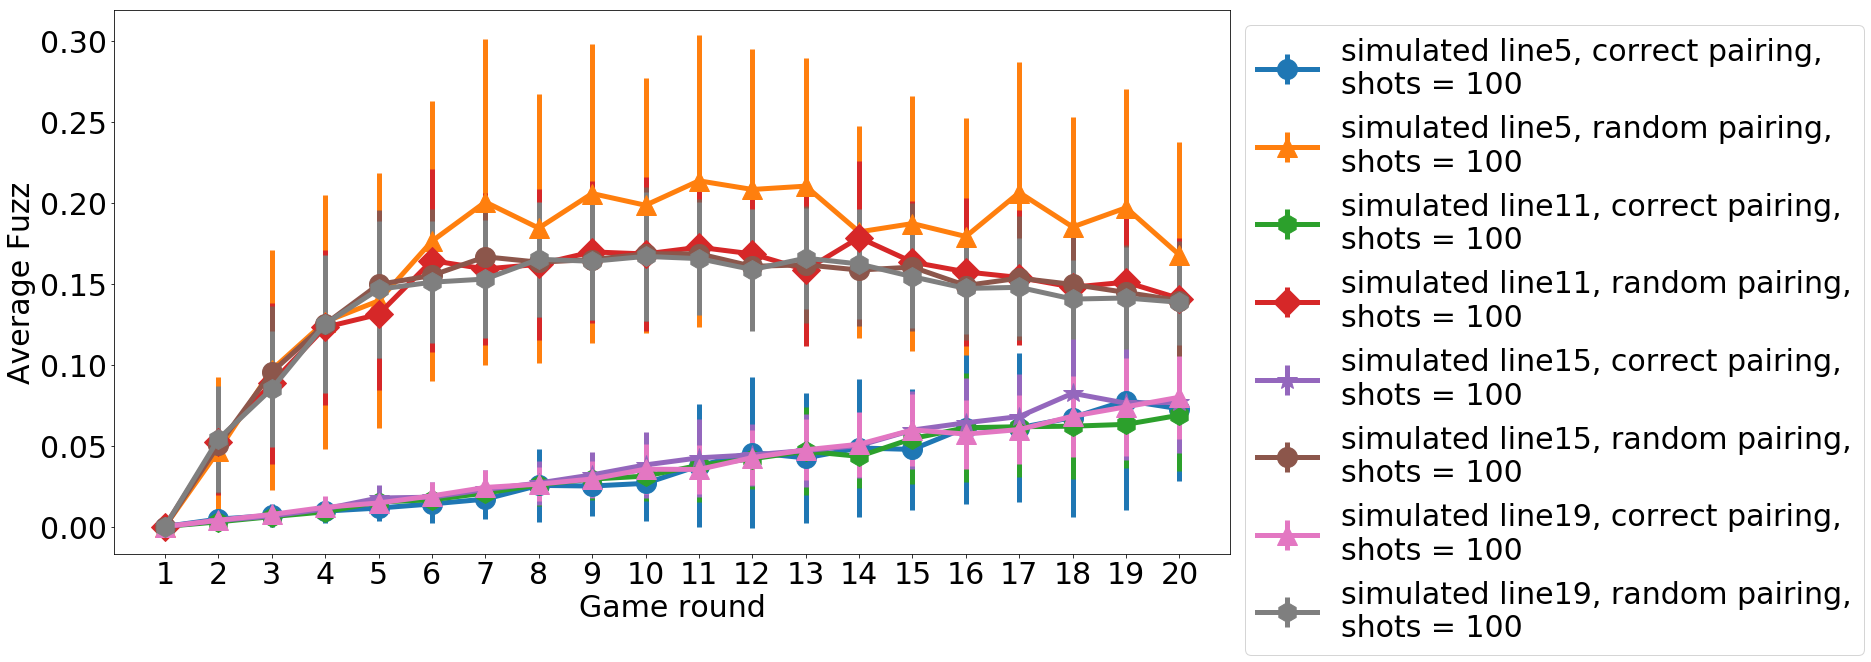
\includegraphics[width=0.9\textwidth]{figures/line_fuzz.png}
    \end{subfigure}
    \begin{subfigure}[b]{\textwidth}
        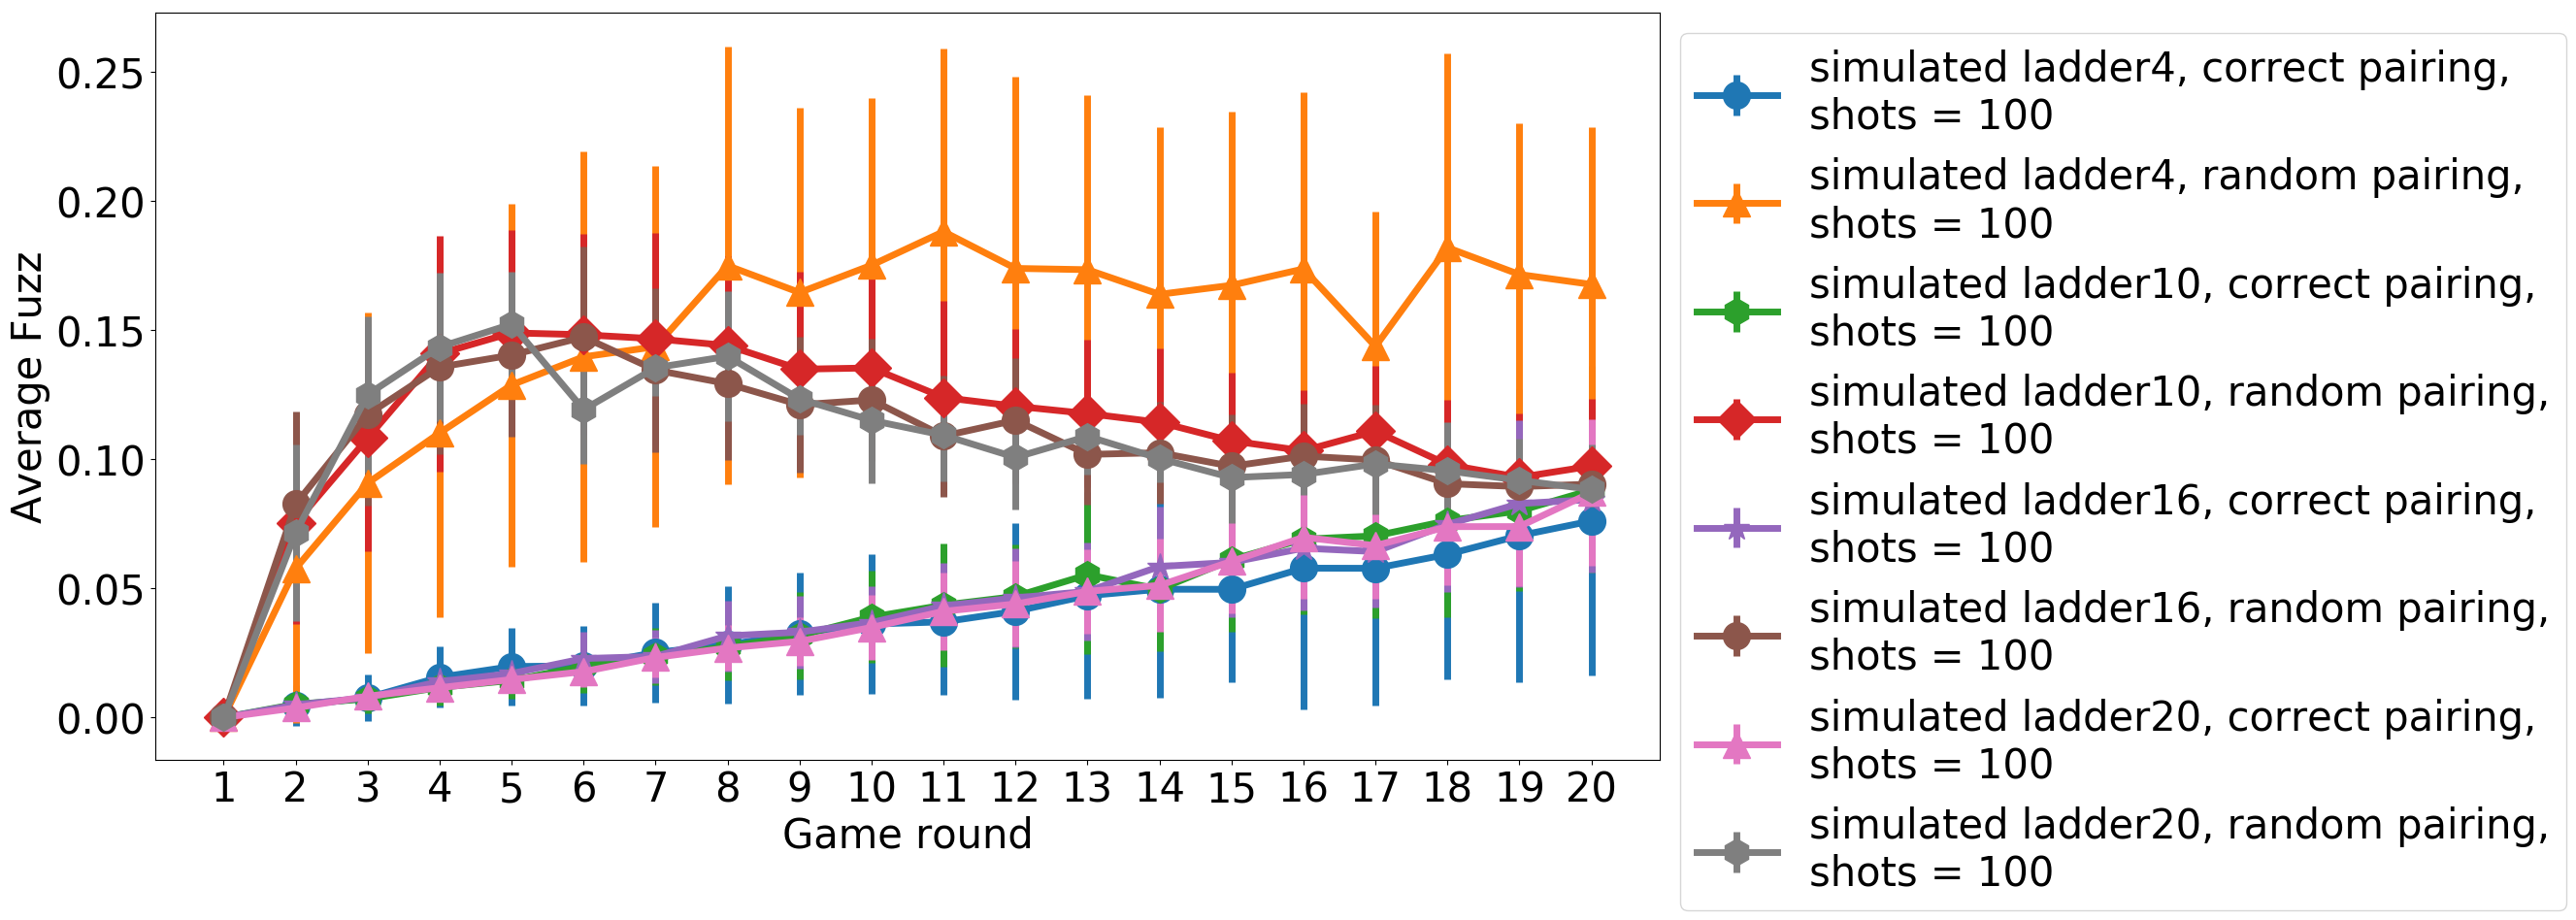
\includegraphics[width=0.9\textwidth]{figures/ladder_fuzz.png}
    \end{subfigure}
    \begin{subfigure}[b]{\textwidth}
        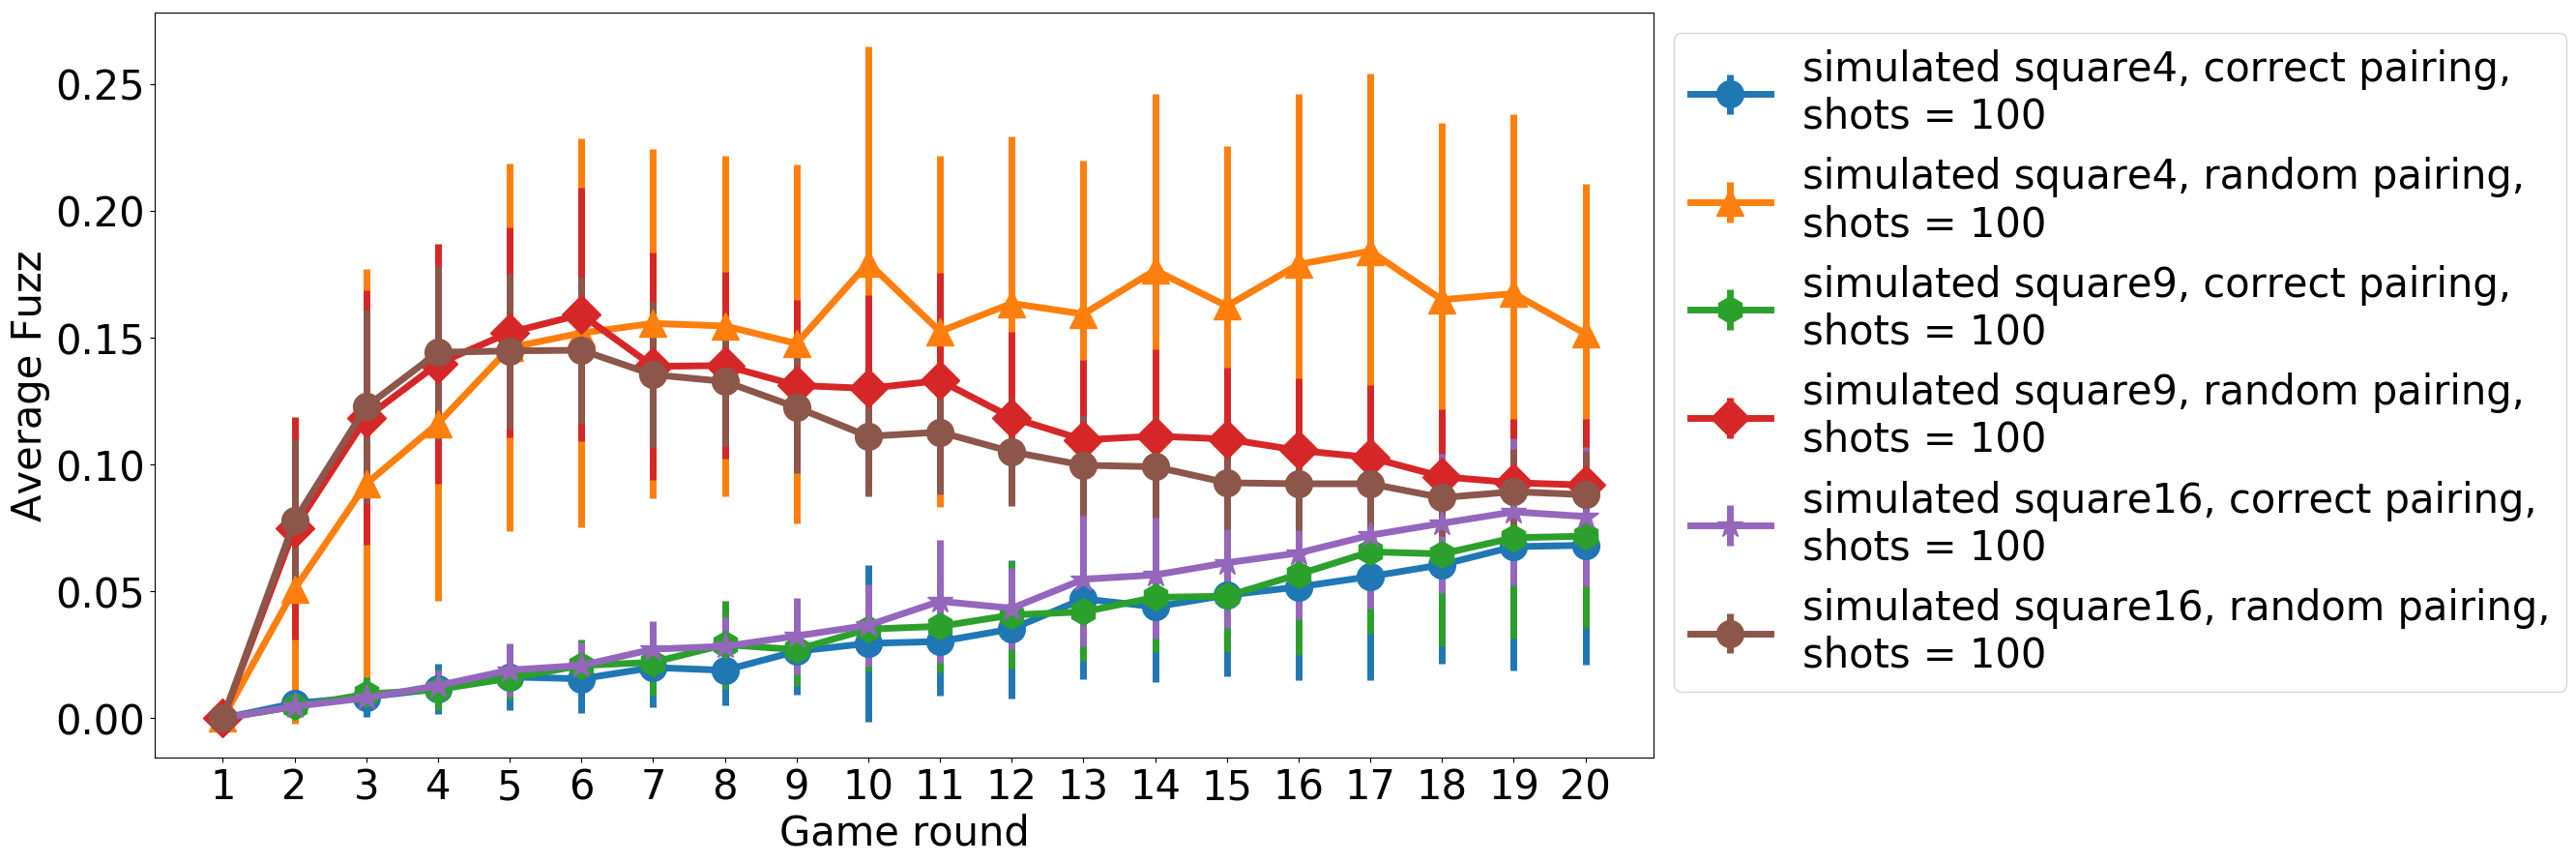
\includegraphics[width=0.9\textwidth]{figures/square_fuzz.png}
    \end{subfigure}
    \begin{subfigure}[b]{\textwidth}
        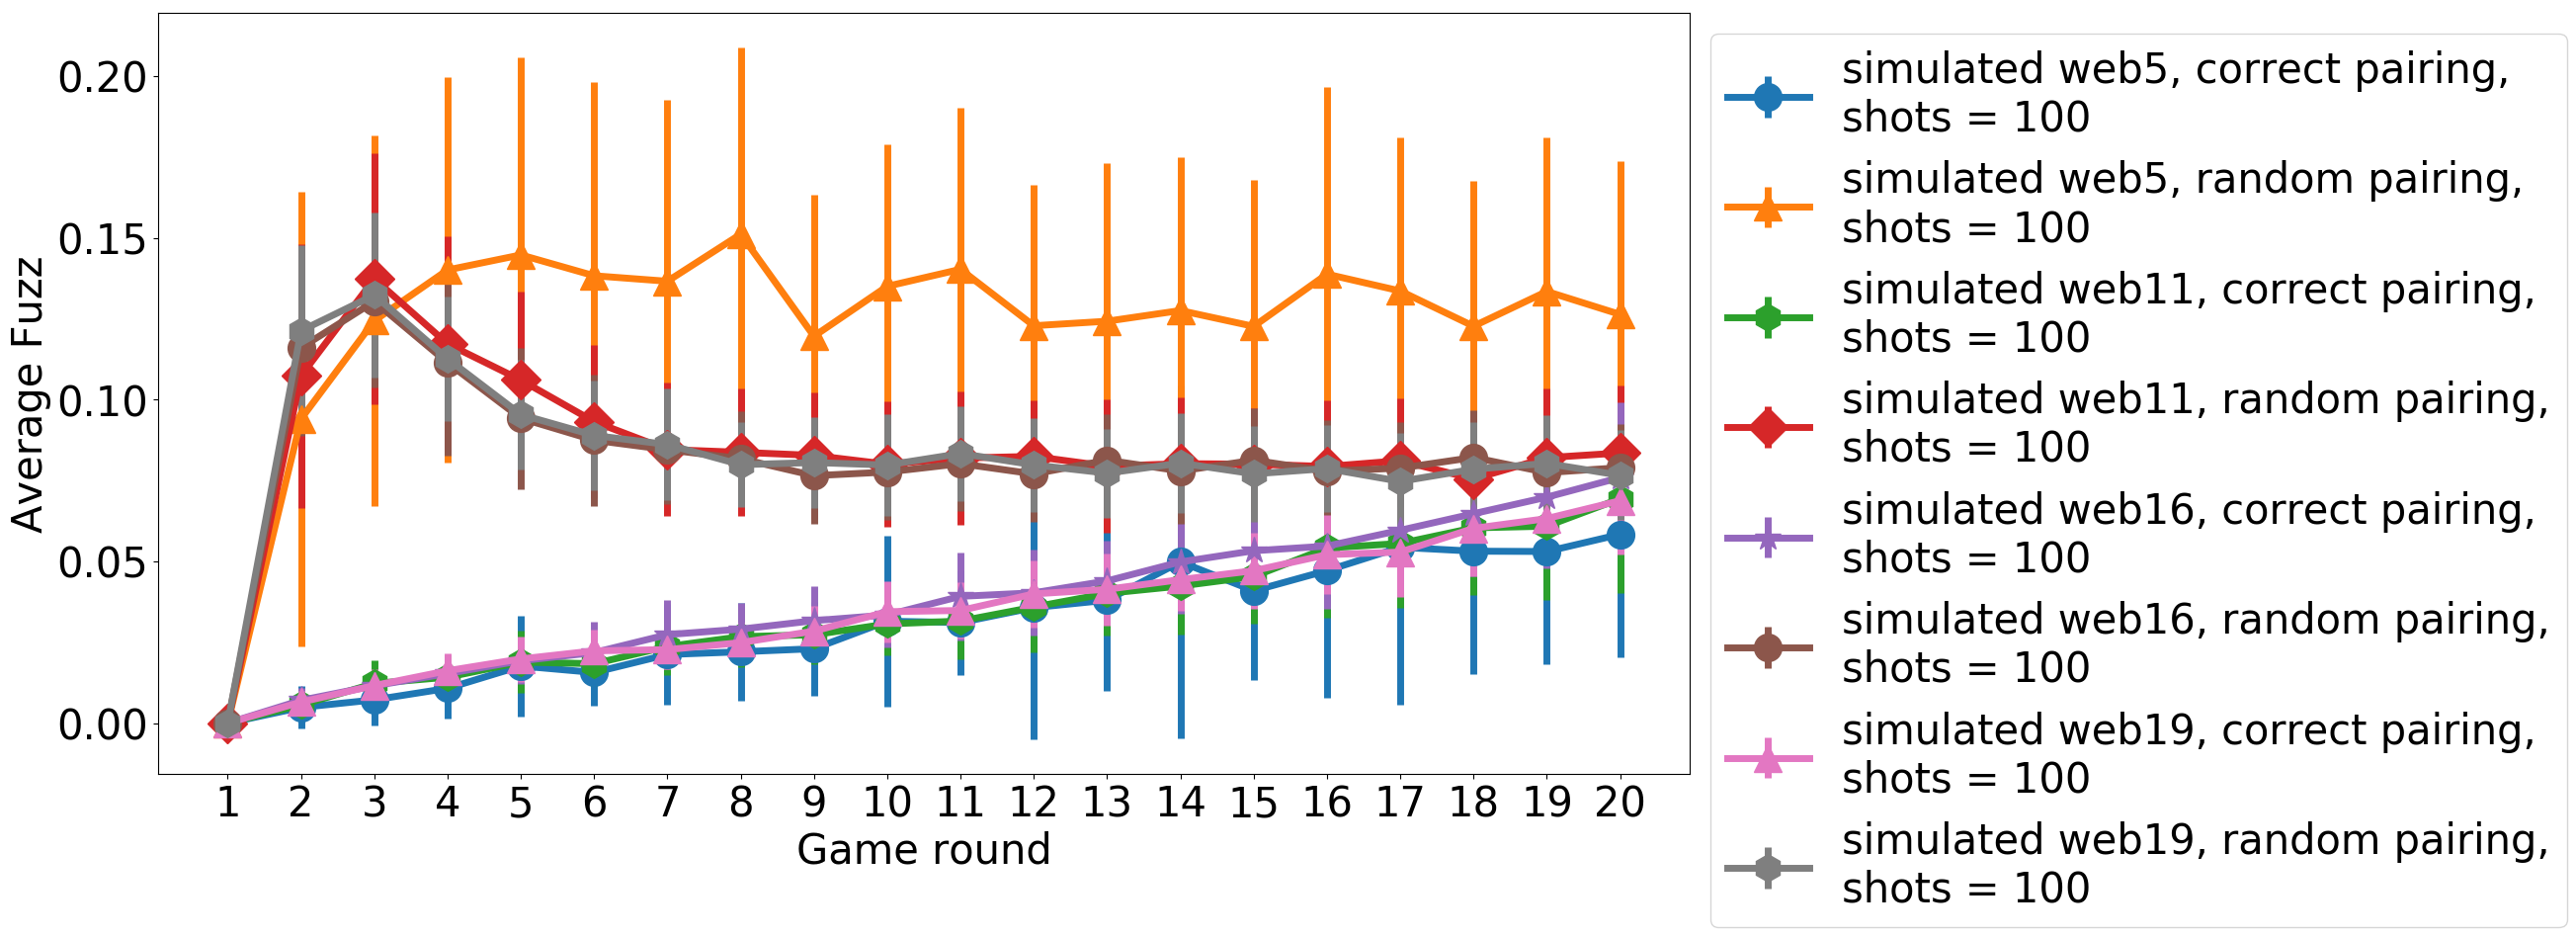
\includegraphics[width=0.9\textwidth]{figures/web_fuzz.png}
    \end{subfigure}
    \caption{The average fuzz for all example devices. Each point is the average of 100 samples, with error bars given by the standard deviation.}\label{fig:example_fuzz}
\end{figure*}

\begin{figure*}
    \centering
    \begin{subfigure}[b]{\textwidth}
        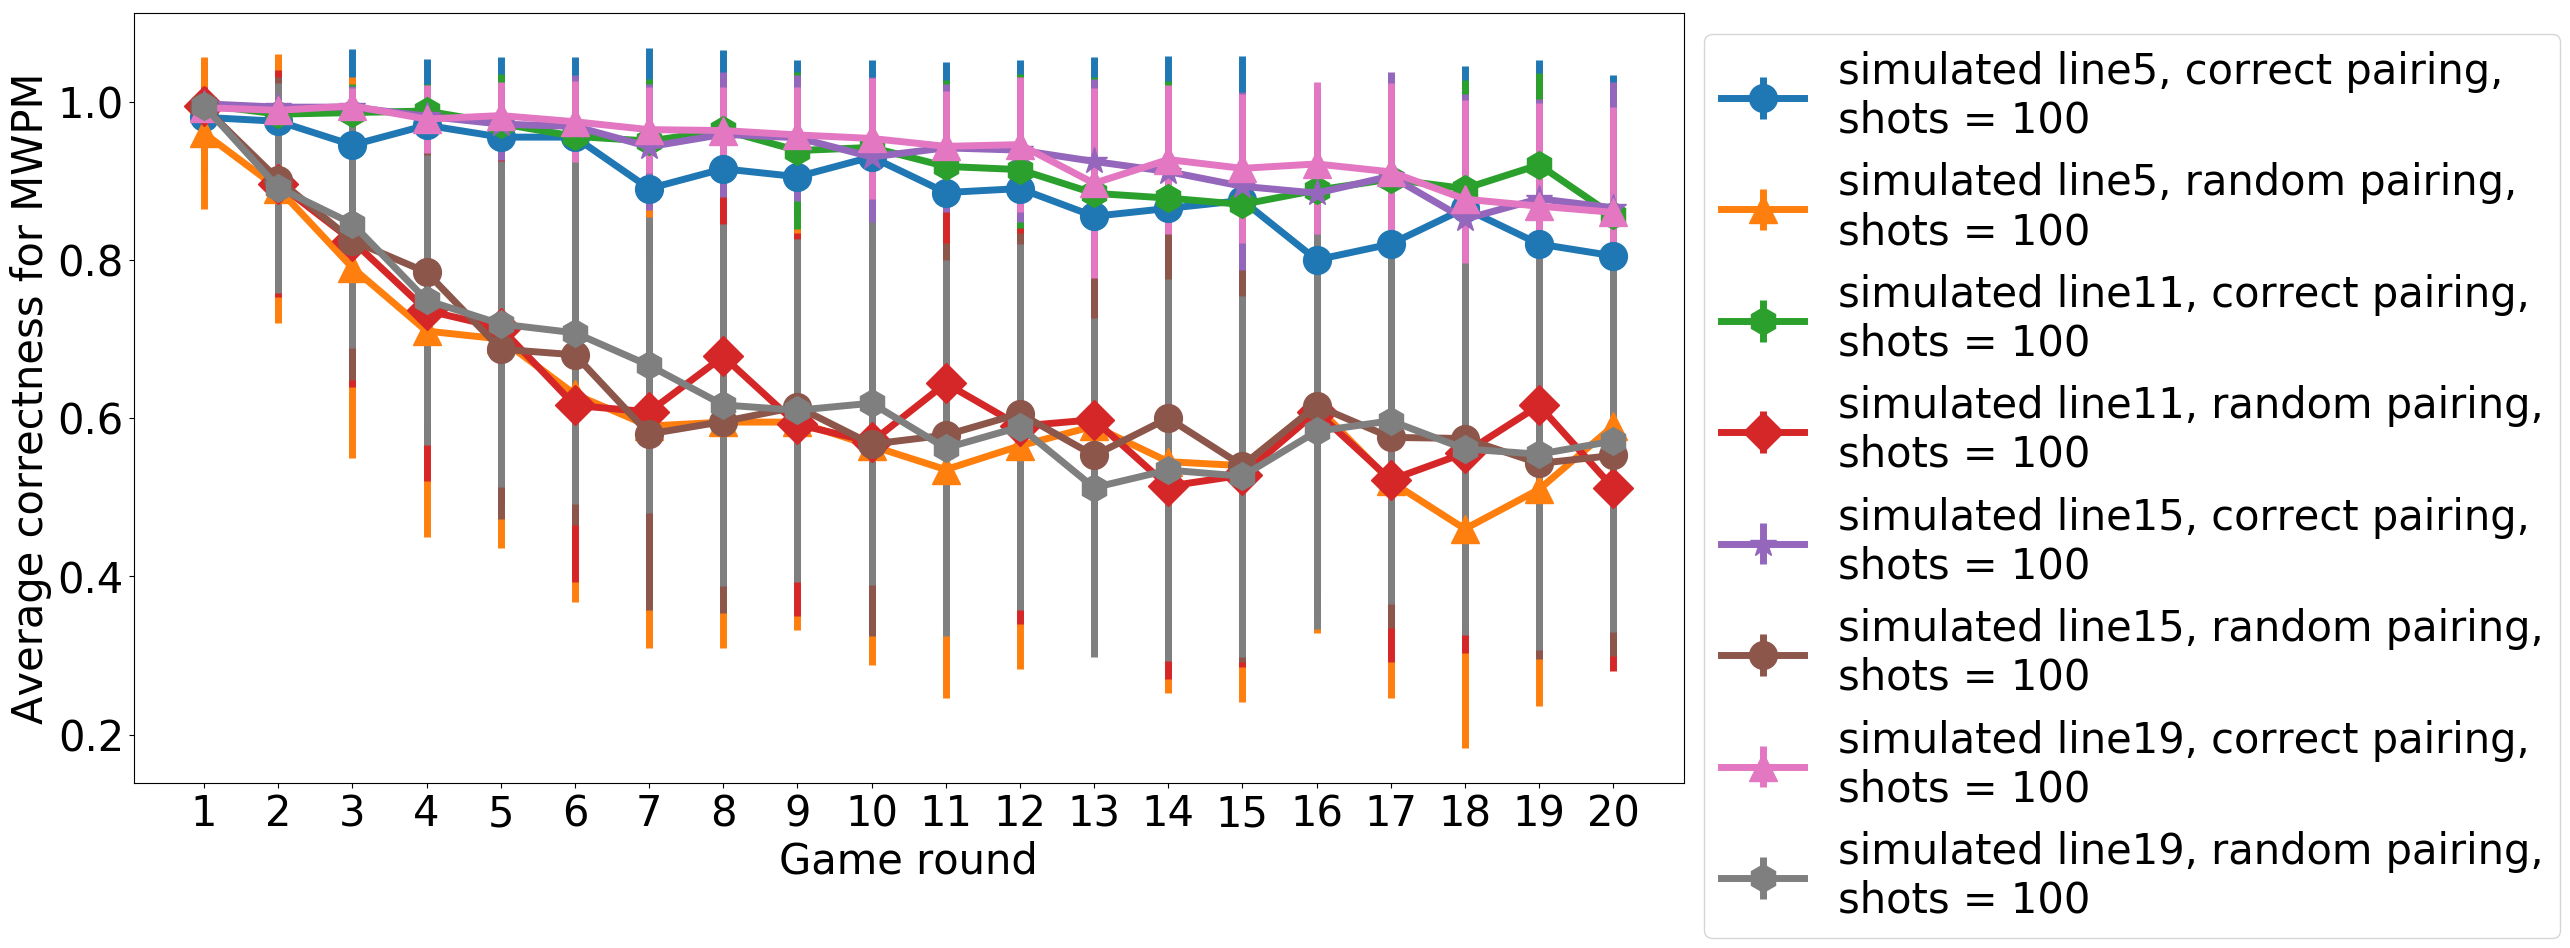
\includegraphics[width=0.9\textwidth]{figures/line_mwpm.png}
    \end{subfigure}
    \begin{subfigure}[b]{\textwidth}
        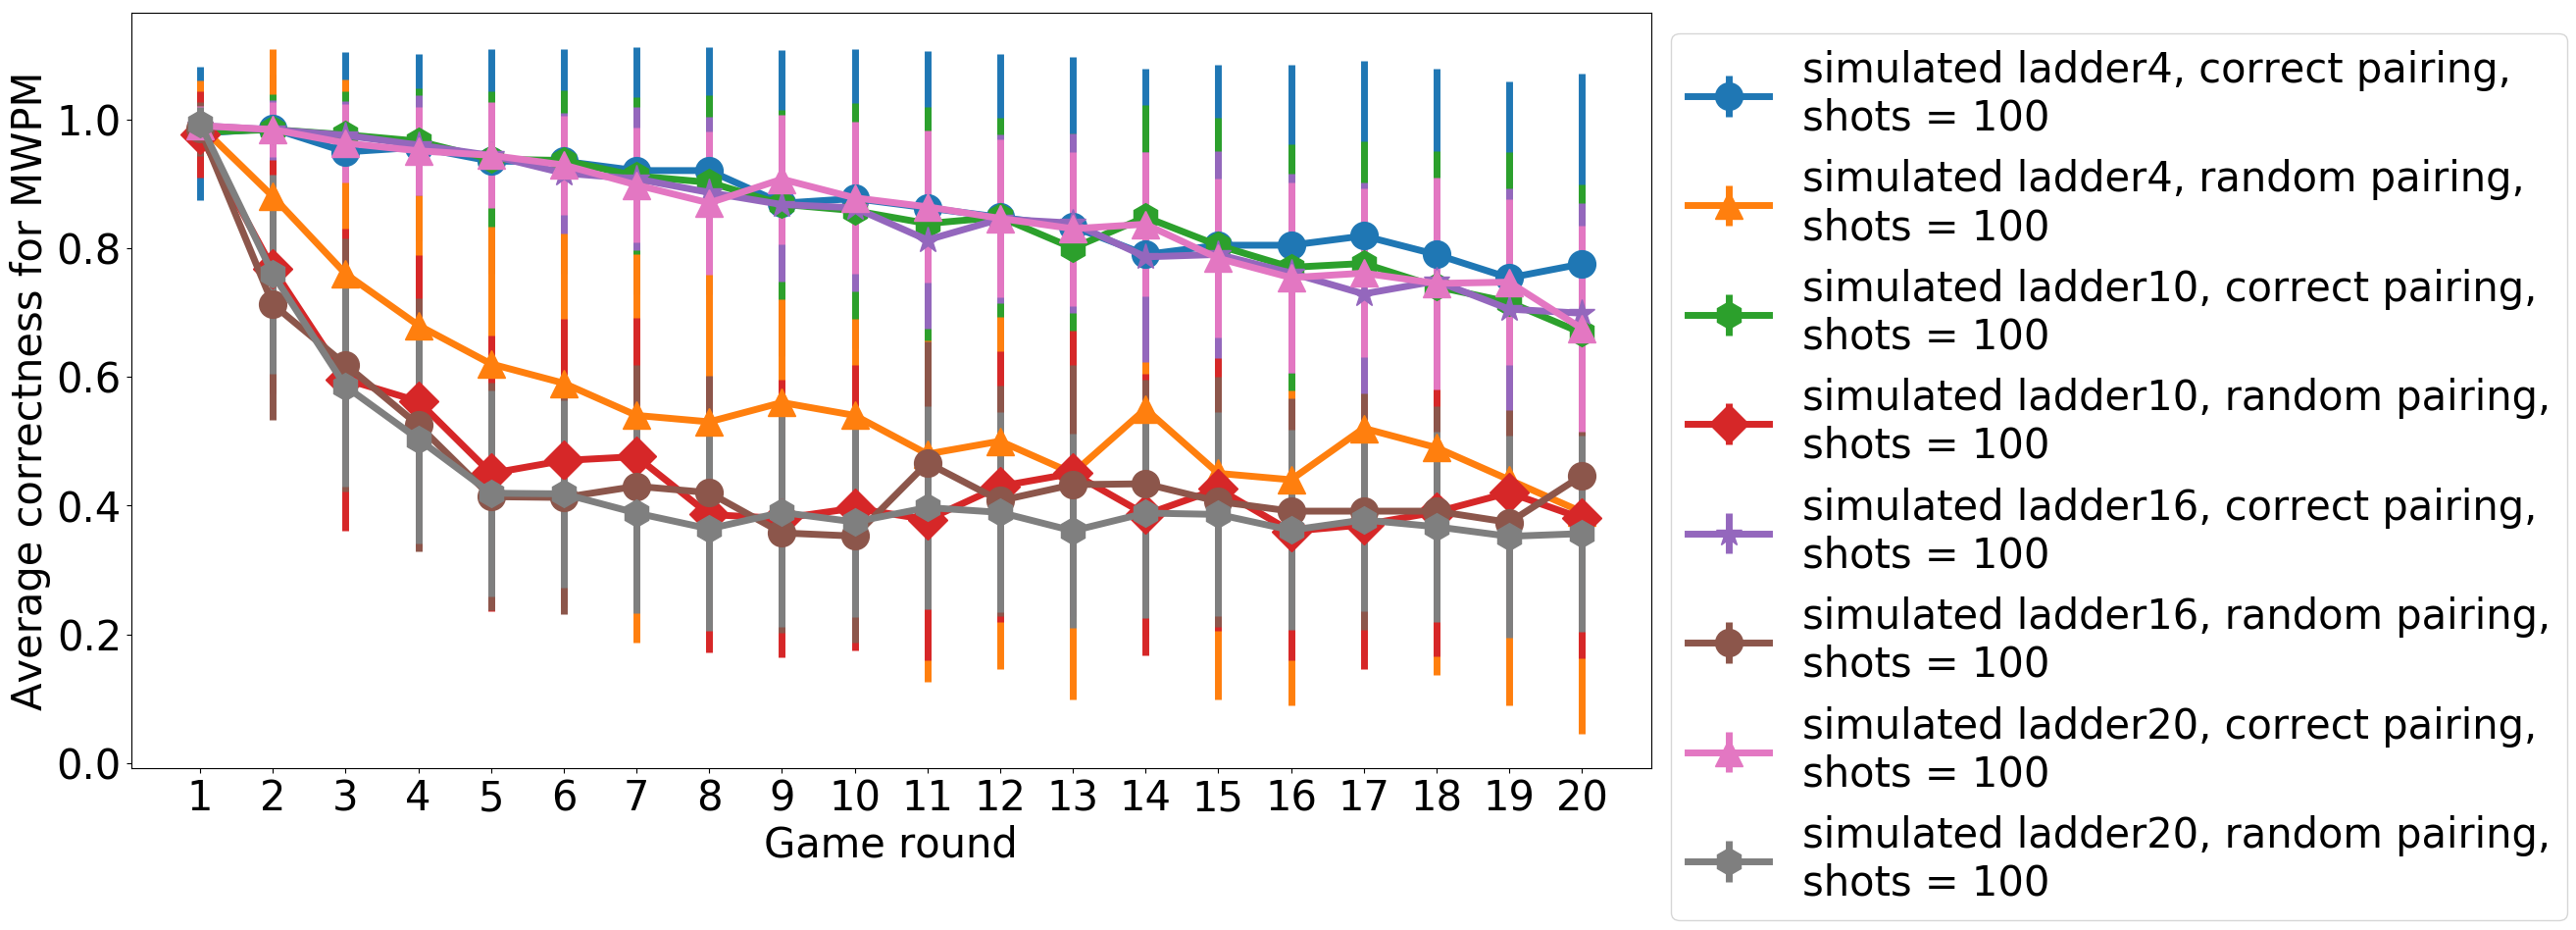
\includegraphics[width=0.9\textwidth]{figures/ladder_mwpm.png}
    \end{subfigure}
    \begin{subfigure}[b]{\textwidth}
        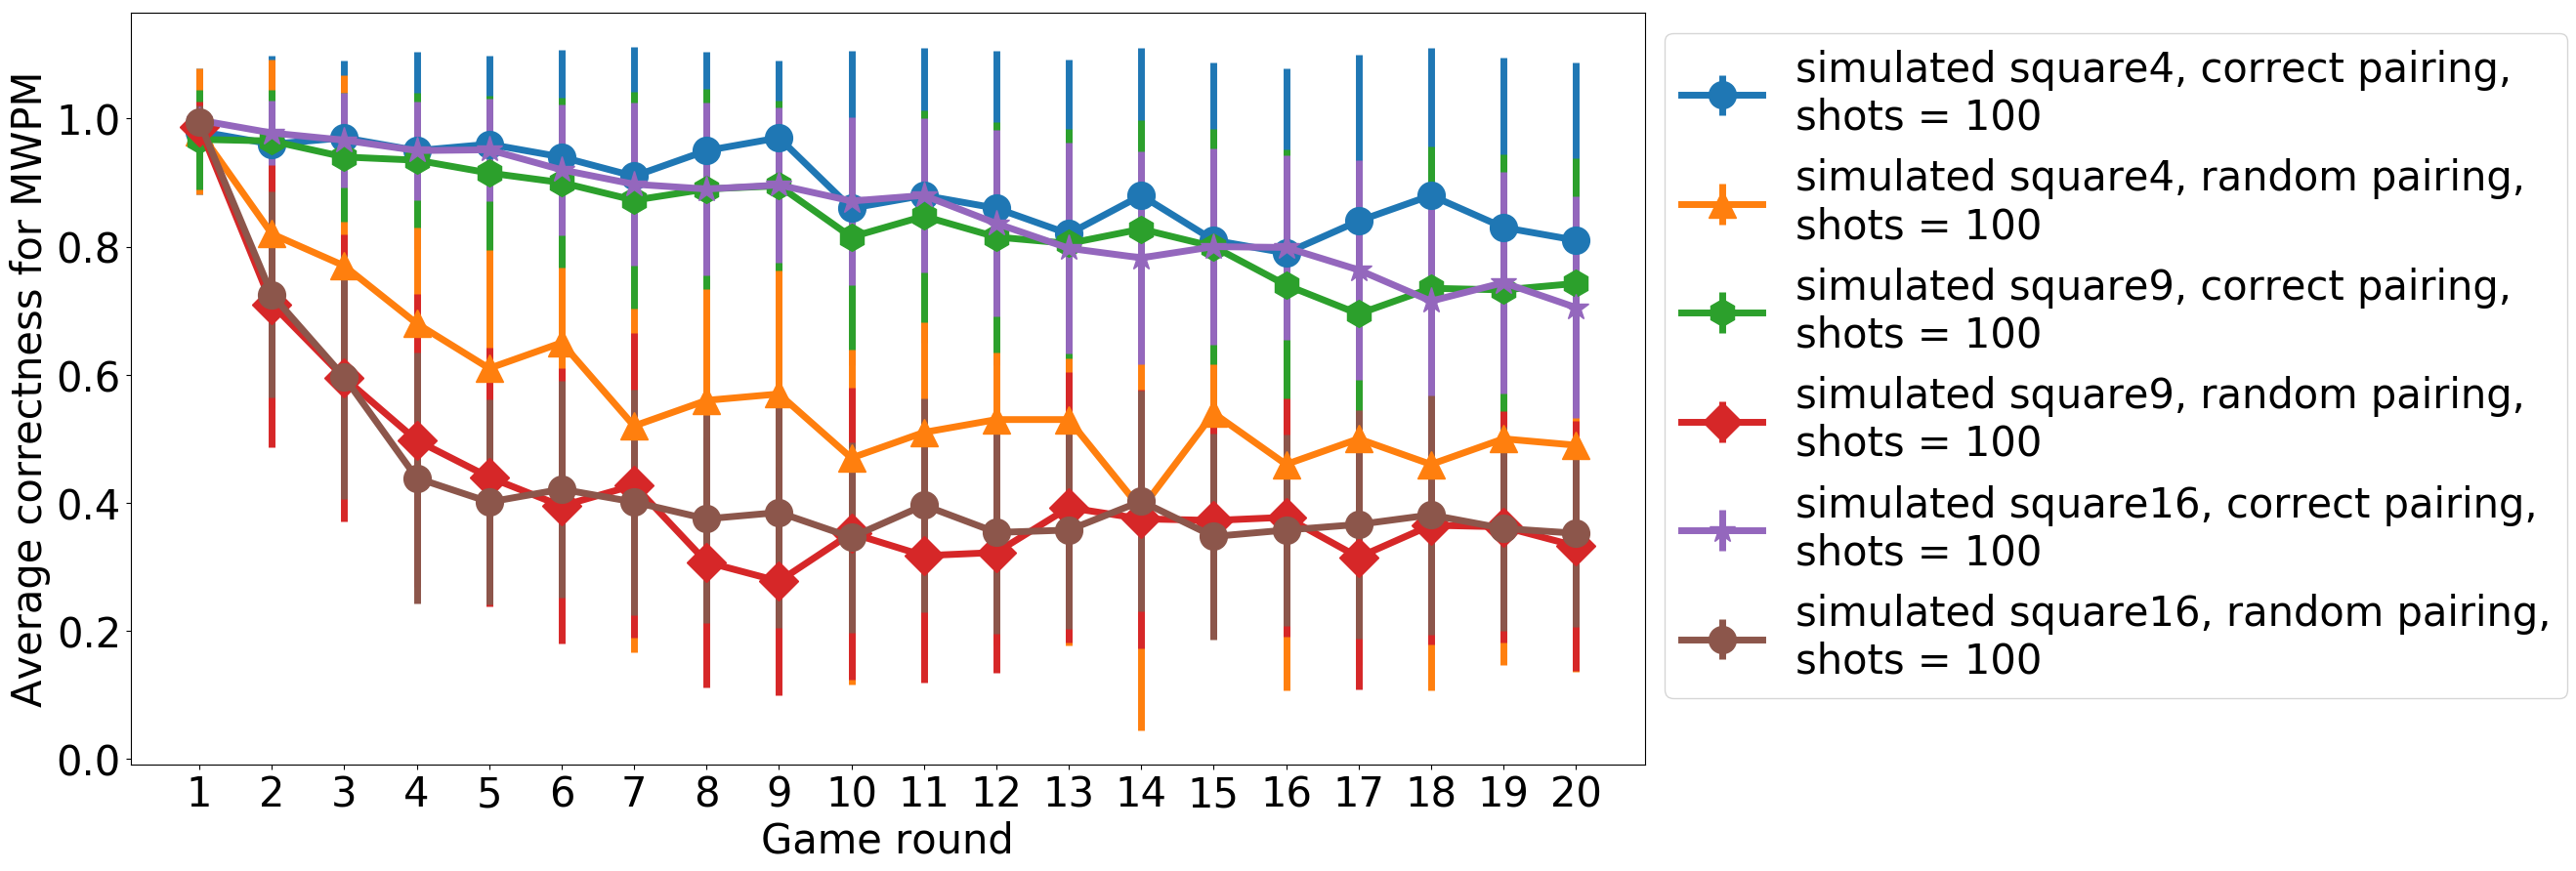
\includegraphics[width=0.9\textwidth]{figures/square_mwpm.png}
    \end{subfigure}
    \begin{subfigure}[b]{\textwidth}
        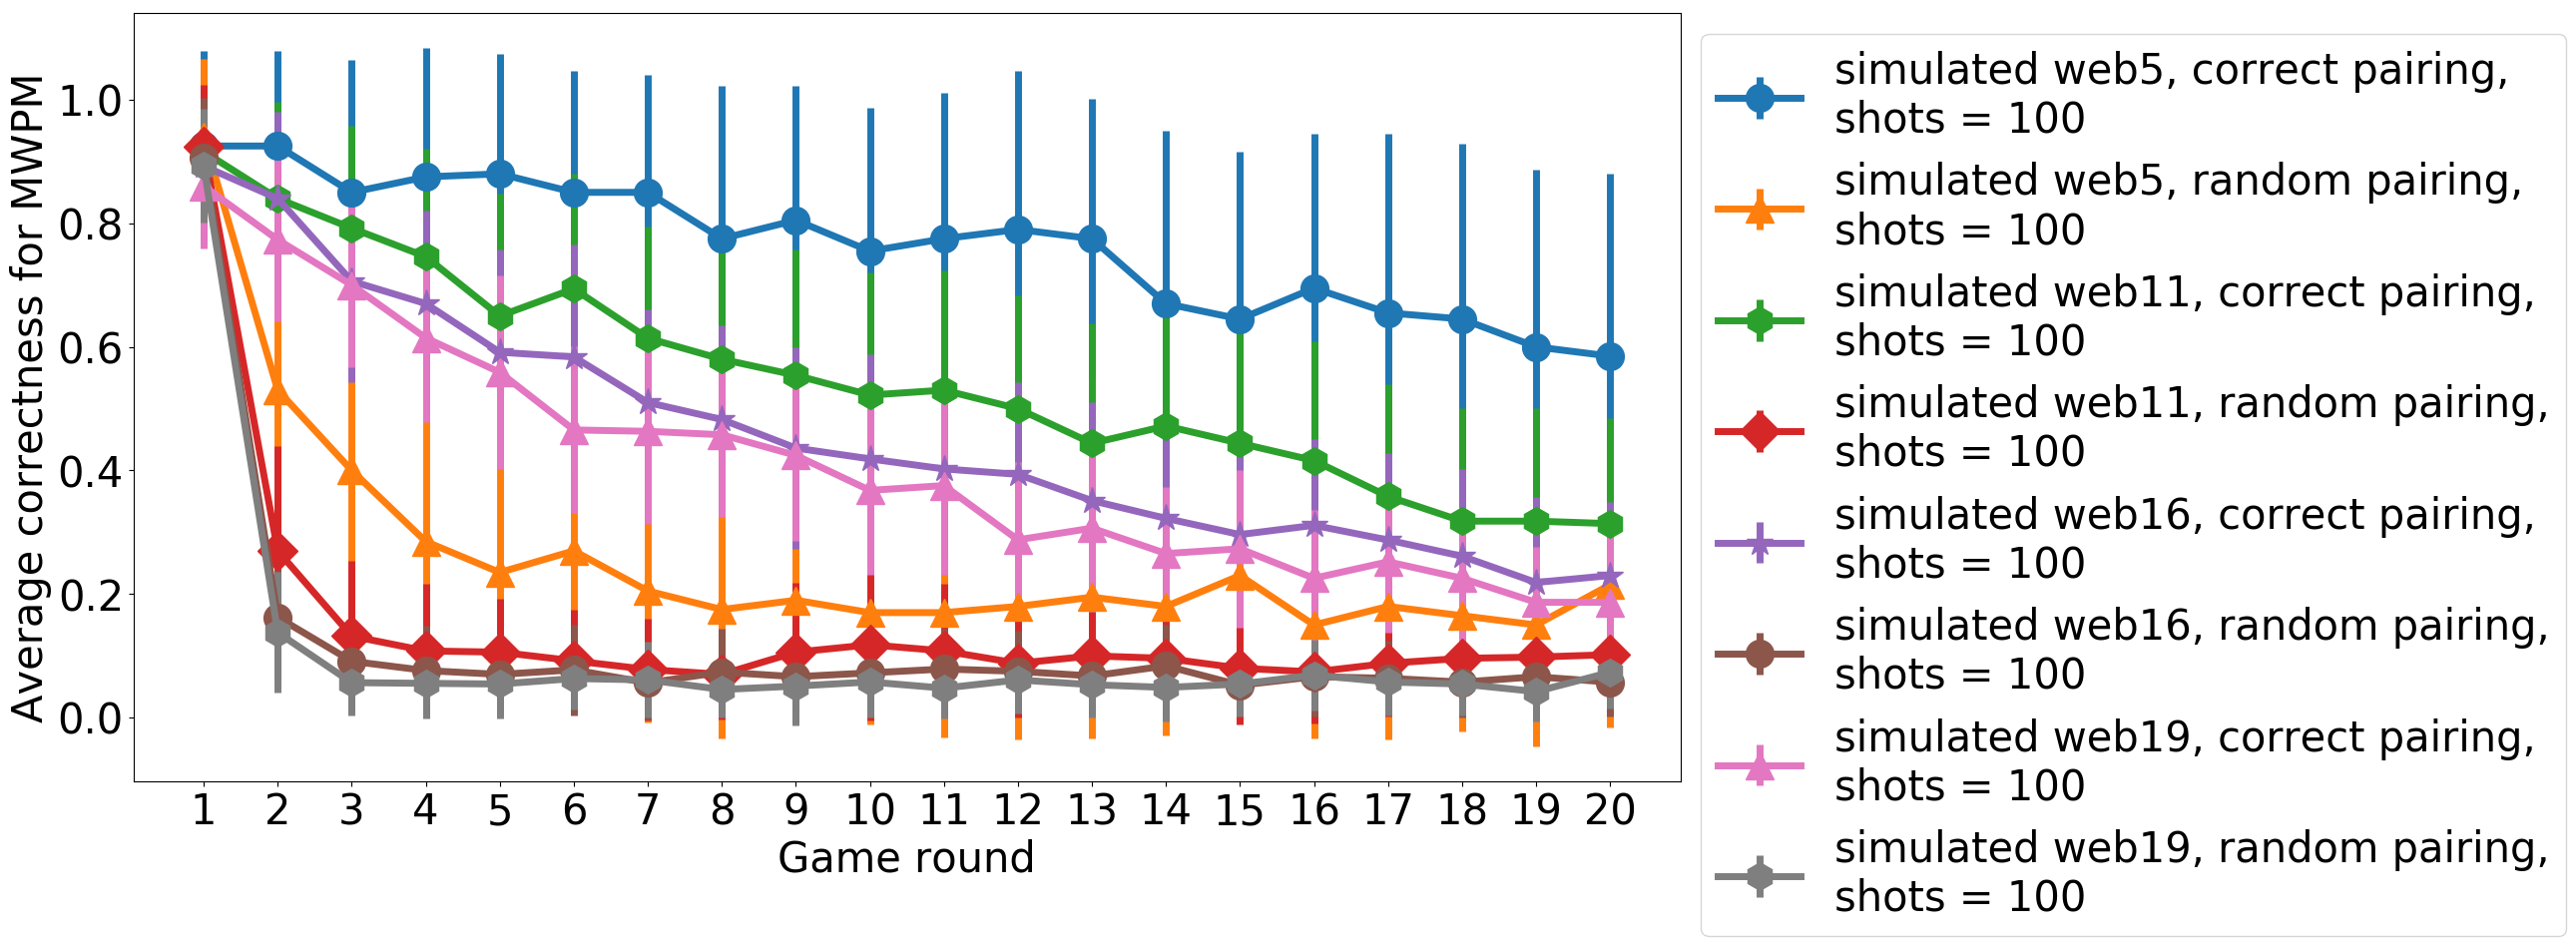
\includegraphics[width=0.9\textwidth]{figures/web_mwpm.png}
    \end{subfigure}
    \caption{The average correctness of pairing via minimum weight perfect matching for all example devices. Each point is the average of 100 samples, with error bars given by the standard deviation.}\label{fig:example_mwpm}
\end{figure*}

\begin{figure*}
    \centering
    \begin{subfigure}[b]{\textwidth}
        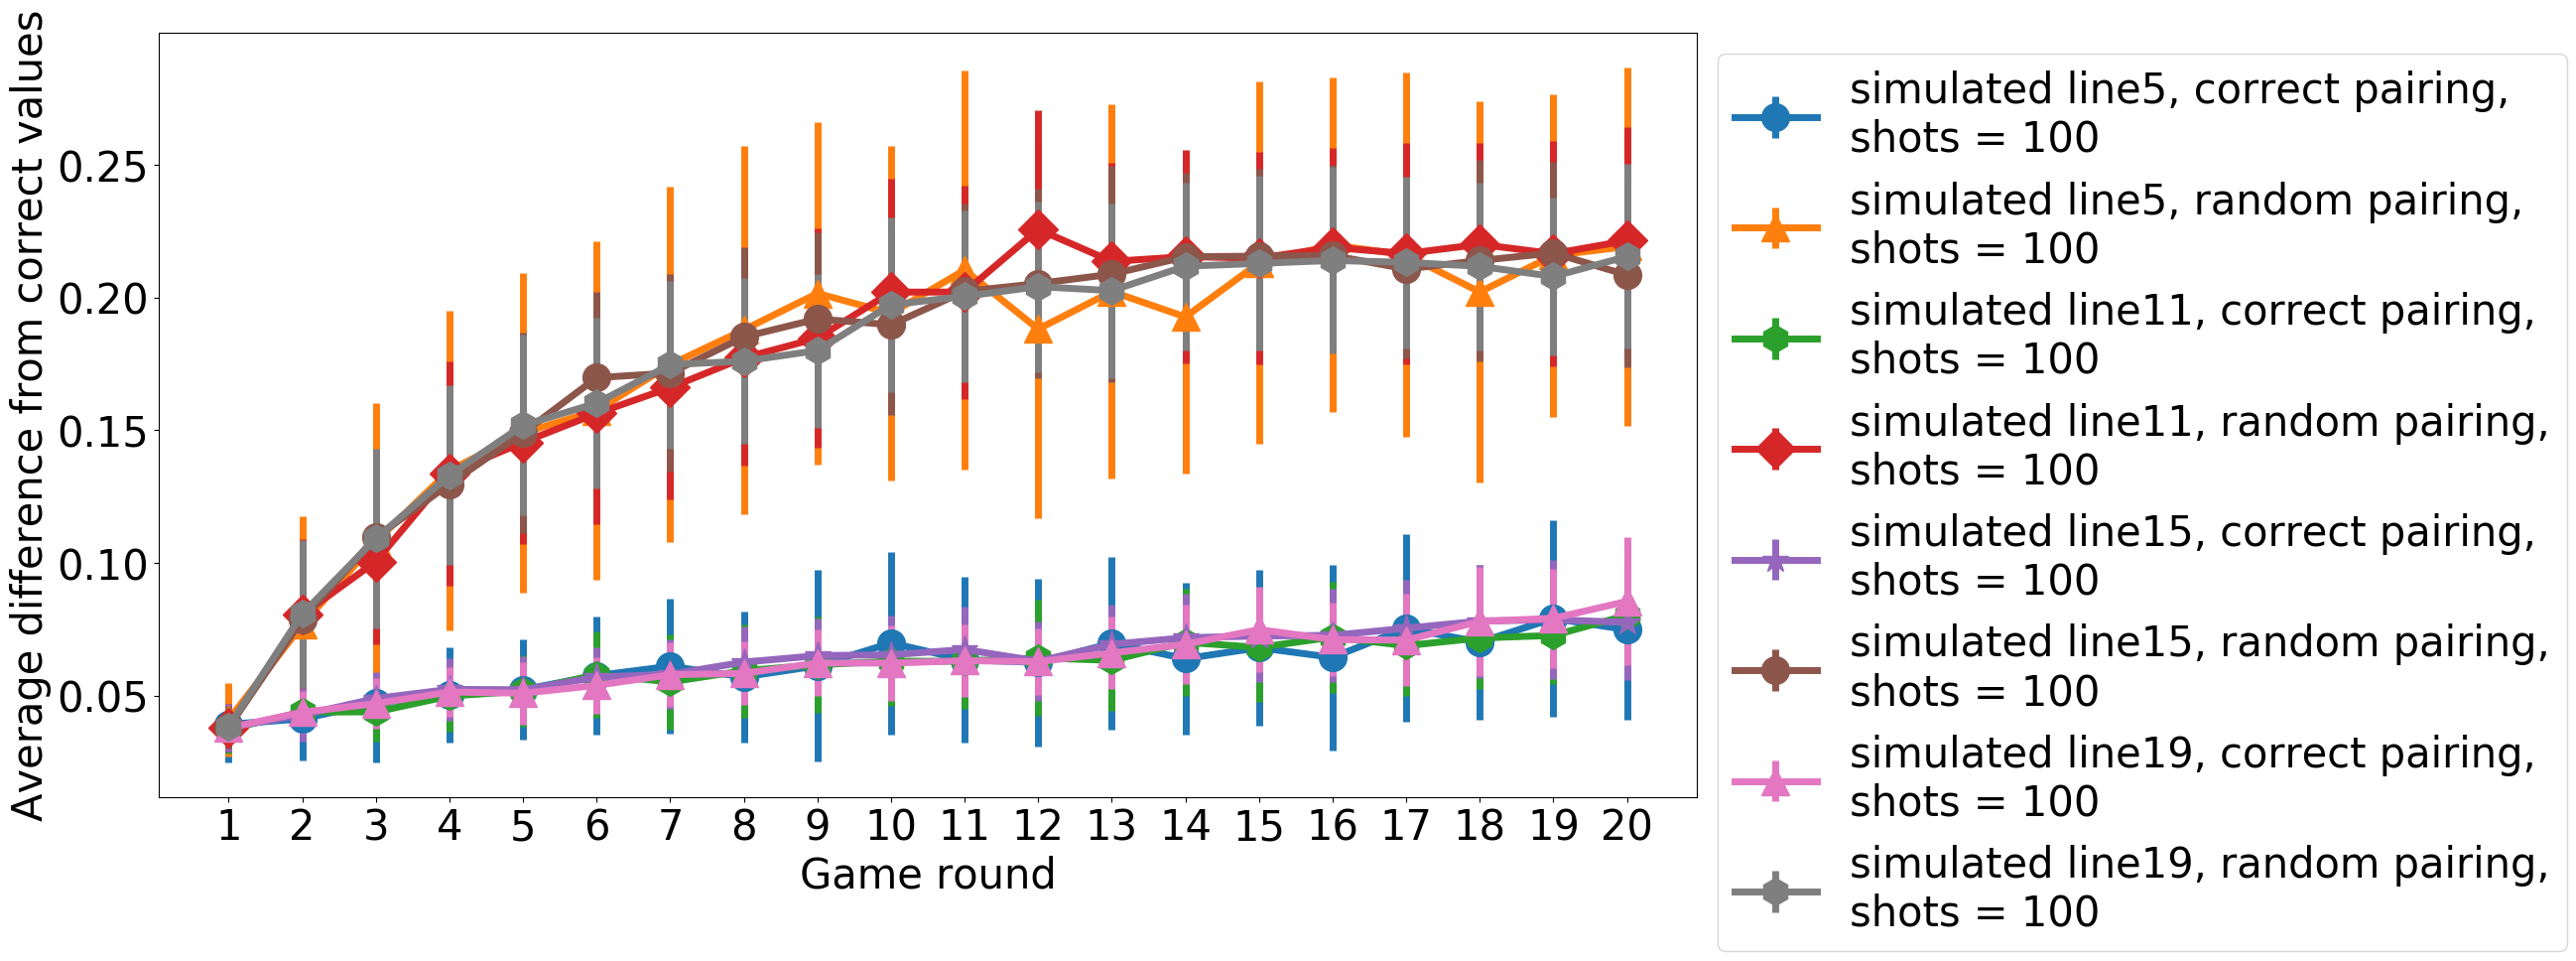
\includegraphics[width=0.9\textwidth]{figures/line_diff.png}
    \end{subfigure}
    \begin{subfigure}[b]{\textwidth}
        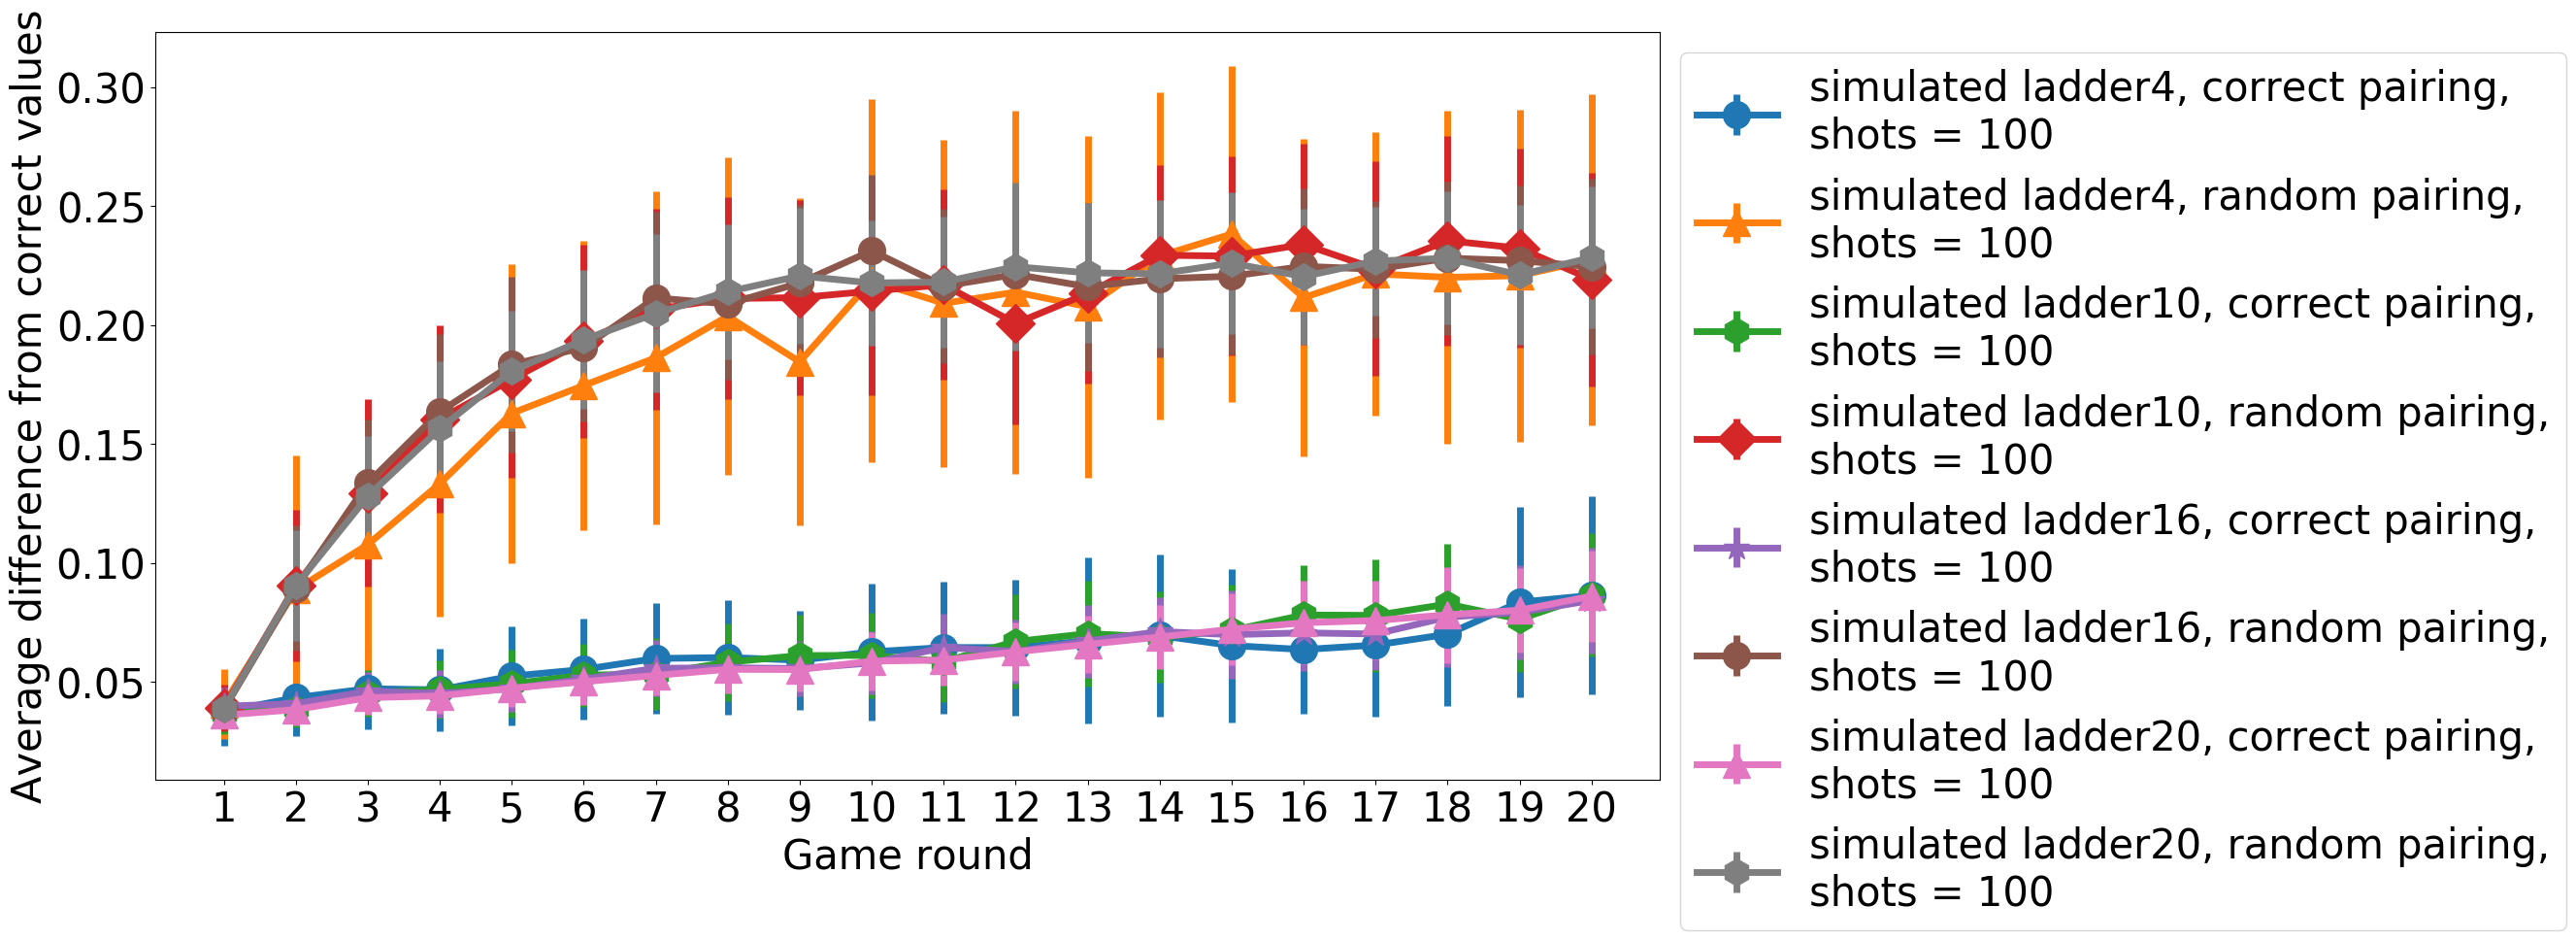
\includegraphics[width=0.9\textwidth]{figures/ladder_diff.png}
    \end{subfigure}
    \begin{subfigure}[b]{\textwidth}
        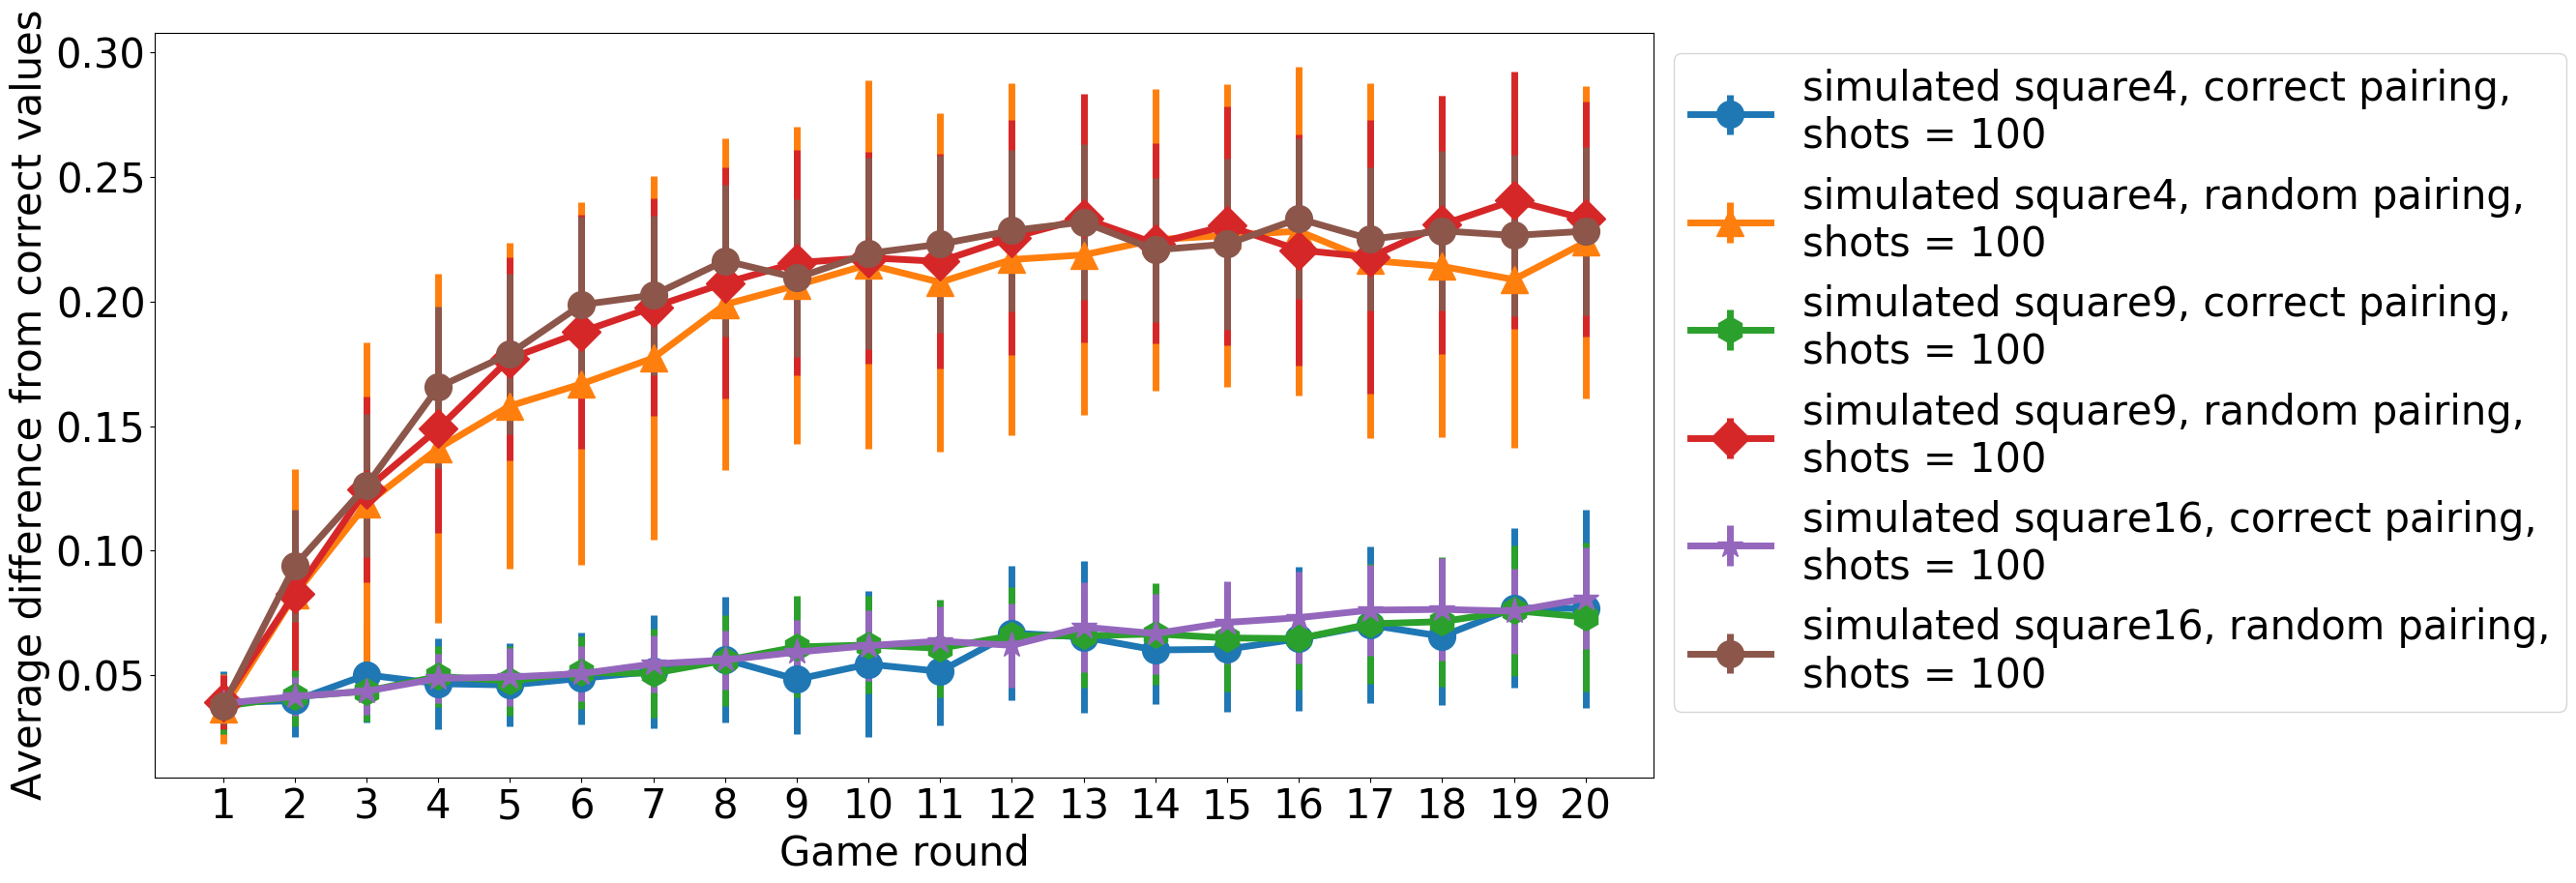
\includegraphics[width=0.9\textwidth]{figures/square_diff.png}
    \end{subfigure}
    \begin{subfigure}[b]{\textwidth}
        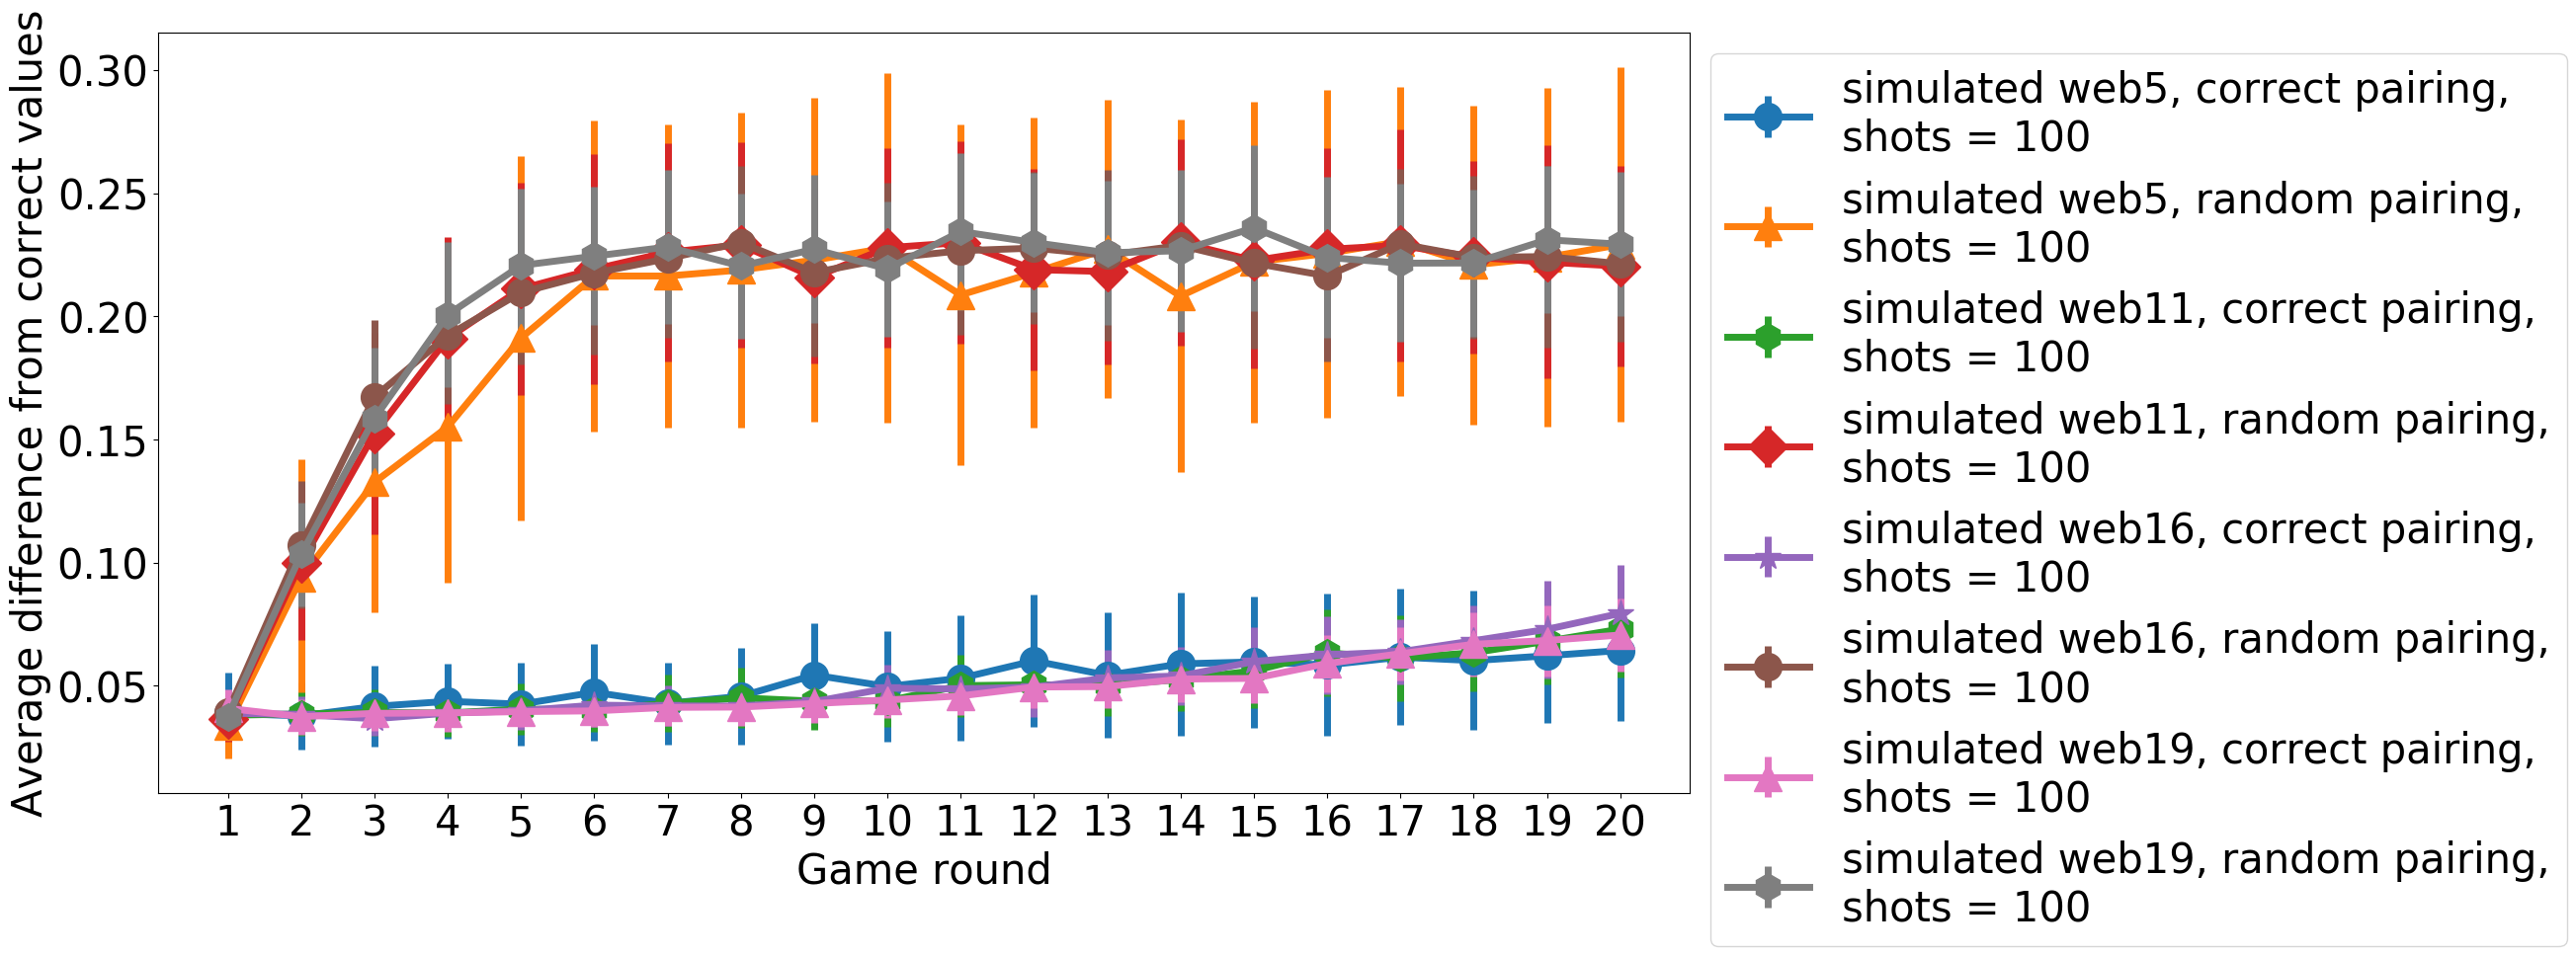
\includegraphics[width=0.9\textwidth]{figures/web_diff.png}
    \end{subfigure}
    \caption{The average difference between inferred and correct values for the $\theta_{jk}$ for all example devices. Each point is the average of 100 samples, with error bars given by the standard deviation.}\label{fig:example_fuzz}
\end{figure*}


\end{document}
